\section{Erweiterung auf Graphen im zweidimensionalen Raum}
\label{raeumliche_erweiterung}

\citeauthor{patchy} haben einen Algorithmus zur Generierung von Receptive-Fields über den Nachbarschaften eines Graphen vorgestellt, der effizient implementiert werden kann und über einer Reihe von Testdatensätzen konkurrenzfähige Resultate im Vergleich zu Methoden, die auf \emph{Graphkernen} basieren, liefert (\vgl{}~\cite{patchy}).
Dabei hängt die Ordnung der Knotenauswahl und der Receptive-Fields stark von einer gewählten Zentralitätsmetrik ab, die auf einem allgemeinen Graphen $\gls{G} = \left(\gls{V}, \gls{E}\right)$ eine fehlende räumliche oder zeitliche Ordnung ersetzt.
Im Kontext von Graphen im zweidimensionalen euklidischen Raum $\gls{G} = \left(\gls{V}, \gls{E}, \gls{p}\right)$, bei denen den Knoten jeweils eine eindeutige Position in der Ebene zugeordnet werden kann, kann die Knotenauswahl $\gls{V}_{\mathrm{out}}$ (Algorithmus~\ref{alg:knotenauswahl}) sowie die Normalisierung der Nachbarschaftsmenge $\gls{N}_{\gls{v}}$ eines Knotens $\gls{v} \in \gls{V}_{\mathrm{out}}$ (Algorithmus~\ref{alg:normalisierung}) diese jedoch folglich berücksichtigen.
Dies erscheint insbesondere dann sinnvoll, wenn sich ein Graph durch viele gleichwertig zentrale Knoten auszeichnet.
So bildet ein Graph, der durch eine \gls{SLIC}-Segmentierung generiert wurde, (in etwa) auf ein unstrukturiertes Gitter ab.
Eine Zentralitätsmetrik auf diesem Graphen besitzt so gut wie keine Aussagekraft.
Der Graph zeichnet sich dabei eher durch seine eindeutige Knotenlage in der Ebene aus.

Die Knotenauswahl wird folglich über die Anordnung der Knoten \bzgl{} ihrer \emph{Scanline}-Ordnung beschrieben, \dhe{} von oben nach unten und von links nach rechts.
Formal lässt sich dafür die Knotenfärbung $\gls{l}_{\mathrm{scanline}} \colon \gls{V} \to \gls{R}$ über
\begin{equation*}
  {\gls{l}_{\mathrm{scanline}}\left(\gls{v}\right)}^{-1} \coloneqq w_{\max} \, {\hat p\left(\gls{v}\right)}_1 + {\hat p\left(\gls{v}\right)}_2
\end{equation*}
mit dem maximalen Breitenabstand $w_{\max} \coloneqq \max_{\gls{v}_i, \gls{v}_j \in \gls{V}} \left({\gls{p}\left(\gls{v}_i\right)}_2 - {\gls{p}\left(\gls{v}_j\right)}_2 \right)$ und der normalisierten Position
\begin{equation*}
  \hat p\left(\gls{v}\right) \coloneqq {\left[\left\lfloor\frac{{\gls{p}\left(\gls{v}\right)}_1 - y_{\min}}{\delta} \right\rfloor, {\gls{p}\left(\gls{v}\right)}_2 - x_{\min}\right]}^{\top}
\end{equation*}
mit $y_{\min} \coloneqq \min \left({\gls{p}\left(\gls{v}_1\right)}_1, \ldots, {\gls{p}\left(\gls{v}_N\right)}_1\right)$ \bzw{} $x_{\min} \coloneqq \min \left({\gls{p}\left(\gls{v}_1\right)}_2, \ldots, {\gls{p}\left(\gls{v}_N\right)}_2\right)$ und $\delta \in \gls{R+}$ definieren, sodass Knoten einen höheren Farbwert erhalten, umso geringer ihre $y$-Koordinate ist und bei annäherend gleicher $y$-Koordinate ihre $x$-Koordinate die Farben weiter differenziert.
Dafür werden die jeweiligen Positionen $\gls{p}\left(\gls{v}\right)$ mittels $\hat p\left(\gls{v}\right)$ in den positiven reellen Raum transformiert.
Die $y$-Koordinate von $\hat p$ wird weiter auf eine über $\delta$ steuerbare natürliche Zahl gerundet.
Dadurch werden kleine Fluktuationen in den $y$-Koordinaten ausgeglichen, die ansonsten eine vollkommen willkürliche Ordnung erzeugen würden.
Die $y$-Koordinate von $\hat p\left(\gls{v}\right)$ wird in $\gls{l}_{\mathrm{scanline}}$ daraufhin insofern gewichtet, dass für zwei unterschiedliche $y$-Koordinaten die Ordnung, die die Knotenfärbung generiert, nicht von der $x$-Koordinate beeinflusst wird.
Damit entspricht der Algorithmus~\ref{alg:knotenauswahl} mit der Knotenfärbung $\gls{l}_{\mathrm{scanline}}$ in etwa der Pixelauswahl einer klassischen Faltung auf regulären Gittern, mit dem Unterschied, dass die Knotenauswahl letztendlich eine eindimensionale geordnete Menge definiert.
Das ist aufgrund der möglichen Irregularitäten in den jeweiligen Knotenpositionen allerdings nicht zu vermeiden.
Folglich sind benachbarte Knoten in $\gls{V}_{\mathrm{out}}$ nicht zwangsläufig auch in der Ebene benachbart.
$\gls{l}_{\mathrm{scanline}}$ generiert jedoch eine Knotenfärbung, die für zwei strukturell gleiche Graphen eine ähnliche Ordnung generiert.

Analog zu einem klassischen \gls{CNN} lässt sich auch die Ordnung des Receptive-Fields \bzw{} die Normalisierung der Nachbarschaftsmenge $\gls{Neighbor}_{\gls{v}}$ eines Knotens $\gls{v} \in \gls{V}_{\mathrm{out}}$ gestalten.
Dafür wird eine Knotenfärbung $\gls{l}_{\gls{v}} \colon \gls{V} \to \gls{R}$ bestimmt, die die Knoten entsprechend ihrer Winkel zum Wurzelknoten $\gls{v} \in \gls{V}$ ordnet.
\begin{figure}[t]
\centering
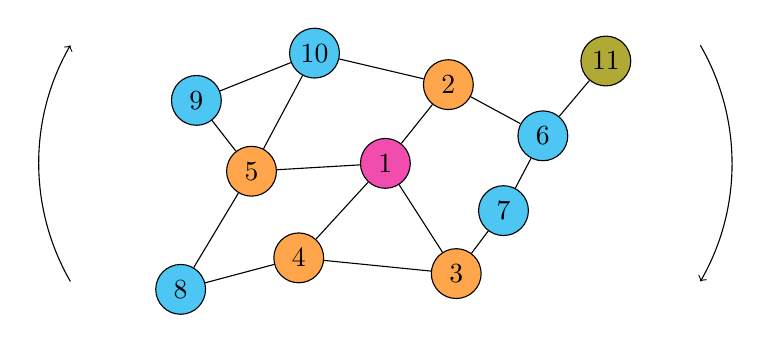
\begin{tikzpicture}
  \tikzstyle{node}=[circle,draw, minimum width=18pt, inner sep=0pt]
  \tikzstyle{root}=[fill=magenta!70]
  \tikzstyle{color1}=[fill=orange!70]
  \tikzstyle{color2}=[fill=cyan!70]
  \tikzstyle{color3}=[fill=olive!70]

  \node[node, root]   (1)  at (0,     0)    {$1$};
  \node[node, color1] (2)  at (0.8,   1)    {$2$};
  \node[node, color1] (3)  at (0.9,   -1.4) {$3$};
  \node[node, color1] (4)  at (-1.1,  -1.2) {$4$};
  \node[node, color1] (5)  at (-1.7,  -0.1) {$5$};
  \node[node, color2] (6)  at (1.5,   -0.6) {$7$};
  \node[node, color2] (7)  at (2,     0.35) {$6$};
  \node[node, color2] (8)  at (-0.9,  1.4)  {$10$};
  \node[node, color2] (9)  at (-2.4,  0.8)  {$9$};
  \node[node, color2] (10) at (-2.6,  -1.6) {$8$};
  \node[node, color3] (11) at (2.8,   1.3)  {$11$};

  \path (1) edge (2);
  \path (1) edge (3);
  \path (1) edge (4);
  \path (1) edge (5);
  \path (2) edge (7);
  \path (2) edge (8);
  \path (3) edge (4);
  \path (3) edge (6);
  \path (4) edge (10);
  \path (5) edge (8);
  \path (5) edge (9);
  \path (5) edge (10);
  \path (6) edge (7);
  \path (7) edge (11);
  \path (8) edge (9);

  \draw[<-] (4,  -1.5) arc (-30:30:3);
  \draw[<-] (-4, 1.5)  arc (150:210:3);
\end{tikzpicture}
\caption[Normalisierung für Graphen im zweidimensionalen Raum]{Normalisierung eines Receptive-Fields der Größe $11$ eines Graphen im zweidimensionalen euklidischen Raum.
  Knoten werden basierend \bzgl{} ihrer Pfadlänge zum Wurzelknoten (rot) gruppiert, hier dargestellt über die unterschiedlichen Farbtöne der Knoten.
  In diesen werden die Knoten entsprechend ihrer Winkel zum Wurzelknoten im Uhrzeigersinn geordnetet.}
\label{fig:normalisierung_erweitert}
\end{figure}

Sei dafür $\gls{winkel}_{\gls{v}} \colon \gls{V} \to \left(0, 2\pi\right]$ analog zu~\eqref{eq:winkelfunktion} gegeben als
\begin{equation*}
  \gls{winkel}_{\gls{v}}\left(\gls{v}_i\right) \coloneqq \mathrm{atan2}\left({\gls{p}\left(\gls{v}_i\right)}_1 - {\gls{p}\left(\gls{v}\right)}_1, {\gls{p}\left(\gls{v}_i\right)}_2 - {\gls{p}\left(\gls{v}\right)}_2\right) + \pi.
\end{equation*}
Dann kann $\gls{l}_{\gls{v}}$ \bzgl{} eines Wurzelknotens $\gls{v} \in \gls{V}$ über
\begin{equation*}
  {\gls{l}_{\gls{v}}\left(\gls{v}_i\right)}^{-1} \coloneqq \frac{d_{\max}}{\gls{winkel}_{\min}} \gls{winkel}_{\gls{v}}\left(\gls{v}_i\right) + {\left\|\gls{p}\left(\gls{v}_i\right) - \gls{p}\left(\gls{v}\right)\right\|}_2
\end{equation*}
definiert werden, wobei $d_{\max} \coloneqq \max_{\gls{v}_i \in \gls{V}} {\left\| \gls{p}\left(\gls{v}_i\right) - \gls{p}\left(\gls{v}\right) \right\|}_2$ den maximalen Abstand eines Knotens zum Wurzelknoten und $\gls{winkel}_{\min} \coloneqq \min_{\gls{v}_i, \gls{v}_j \in \gls{V},\, \gls{winkel}_{\gls{v}}\left(\gls{v}_i\right) \neq \gls{winkel}_{\gls{v}}\left(\gls{v}_j \right)} \left|\gls{winkel}_{\gls{v}}\left(\gls{v}_i\right) - \gls{winkel}_{\gls{v}}\left(\gls{v}_j\right)\right|$ den minimalen, echt positiven Winkelabstand zweier Knoten beschreibt.
Damit werden Knoten entsprechend ihrer Winkel zum Wurzelknoten \gls{v} sortiert.
Besitzen zwei Knoten den exakt gleichen Winkel, wird über den Abstand ihrer Positionen zum Wurzelknoten der Farbwert weiter differenziert.
Die Gewichtung des Winkels über $d_{\max}/\gls{winkel}_{\min}$ sorgt dafür, dass für zwei unterschiedliche Winkel $\gls{winkel}_{\gls{v}}\left(\gls{v}_i\right) \neq \gls{winkel}_{\gls{v}}\left(\gls{v}_j\right)$ die Distanzen der Knoten zum Wurzelknoten keinen Einfluss nehmen.

Damit ist $\gls{l}_{\gls{v}}$ für alle Graphen injektiv, für die die Positionsfunktion \gls{p} injektiv ist.
Folglich verfällt bei einer injektiven Positionsabbildung insbesondere die Notwendigkeit der Berechnung einer kanonischen Ordnung des Teilgraphs (\vgl{} Algorithmus~\ref{alg:normalisierung}).
Mit der Einschränkung, dass für $\gls{G}\left(\gls{V}, \gls{E}, \gls{p}\right)$ keine zwei Knoten auf eine gleiche Position abgebildet werden, können damit niemals Äquivalenzen in der Knotenfärbung $\gls{l}_{\gls{v}}$ existieren.
Abbildung~\ref{fig:normalisierung_erweitert} verdeutlicht die entstehende Ordnung, die nach der Anwendung des Normalisierungsalgorithmus~\ref{alg:normalisierung} bei Benutzung von $\gls{l}_{\gls{v}}$ entsteht.

Mit $\gls{l}_{\mathrm{scanline}}$ und $\gls{l}_{\gls{v}}$ stehen uns damit für die Knotenauswahl \bzw{} der Normalisierung zwei Knotenfärbungen zur Verfügung, die uns erlauben, den räumlichen Faltungsoperator auf Graphen im zweidimensionalen euklidischen Raum unter Berücksichtigung ihrer Knotenpositionen zu benutzen.
